\documentclass{article}
\usepackage{amsmath, amsfonts, amssymb, amsthm}
\usepackage{enumitem, tikz}

\title{PS04-01}
\date{\today}

\begin{document}
\maketitle
\begin{enumerate}[label=\alph*.]
	\item When $i \neq 1$, the number of $b$s and $c$s is not important. However, if $i = 1$, then the DFA must output $a^nb^n$, which is not possible, as illustrated by the DFA below. The state $bad$ is where the machine must, but cannot calculate $a^nb^n$.
	\begin{center}
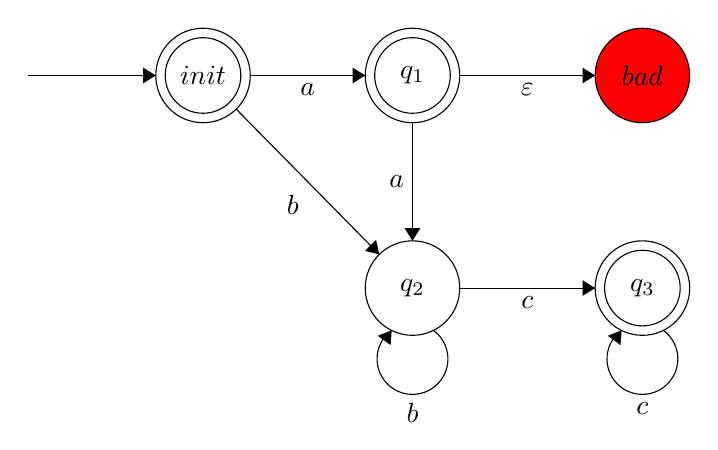
\begin{tikzpicture}[scale=0.2]
\tikzstyle{every node}+=[inner sep=0pt]
\draw [black] (26.7,-22) circle (3);
\draw (26.7,-22) node {$init$};
\draw [black] (26.7,-22) circle (2.4);
\draw [black] (40,-35.5) circle (3);
\draw (40,-35.5) node {$q_2$};
\draw [black] (40,-22) circle (3);
\draw [black] (40,-22) circle (2.4);
\draw (40,-22) node {$q_1$};
\draw [black,fill=red] (54.6,-22) circle (3);
\draw (54.6,-22) node {$bad$};
\draw [black] (54.6,-35.5) circle (3);
\draw (54.6,-35.5) node {$q_3$};
\draw [black] (54.6,-35.5) circle (2.4);
\draw [black] (15.6,-22) -- (23.7,-22);
\fill [black] (23.7,-22) -- (22.9,-21.5) -- (22.9,-22.5);
\draw [black] (28.81,-24.14) -- (37.89,-33.36);
\fill [black] (37.89,-33.36) -- (37.69,-32.44) -- (36.98,-33.14);
\draw (32.82,-30.22) node [left] {$b$};
\draw [black] (41.323,-38.18) arc (54:-234:2.25);
\draw (40,-42.75) node [below] {$b$};
\fill [black] (38.68,-38.18) -- (37.8,-38.53) -- (38.61,-39.12);
\draw [black] (29.7,-22) -- (37,-22);
\fill [black] (37,-22) -- (36.2,-21.5) -- (36.2,-22.5);
\draw (33.35,-22.5) node [below] {$a$};
\draw [black] (40,-25) -- (40,-32.5);
\fill [black] (40,-32.5) -- (40.5,-31.7) -- (39.5,-31.7);
\draw (39.5,-28.75) node [left] {$a$};
\draw [black] (43,-22) -- (51.6,-22);
\fill [black] (51.6,-22) -- (50.8,-21.5) -- (50.8,-22.5);
\draw (47.3,-22.5) node [below] {$\varepsilon$};
\draw [black] (43,-35.5) -- (51.6,-35.5);
\fill [black] (51.6,-35.5) -- (50.8,-35) -- (50.8,-36);
\draw (47.3,-36) node [below] {$c$};
\draw [black] (55.923,-38.18) arc (54:-234:2.25);
\draw (54.6,-42.75) node [below] {$c$};
\fill [black] (53.28,-38.18) -- (52.4,-38.53) -- (53.21,-39.12);
\end{tikzpicture}
\end{center}

	\item Given $w \in F$ and $w = xyz$, if $\mid xy \mid = 1$, the $x = \varepsilon$ and $y = a$. If you were to pump $y$ any number of times, then the $w = xy^tz \in F$.
	\item The Pumping Lemma is a requirement for a language to be regular but not a guarantee. Let $P$ be a predicate meaning that language $A$ passes the pumping lemma. We know that $\neg P \Rightarrow \neg\text{regular}(A)$, but the equation is not biconditional, as proven by parts $a$ and $b$ above. $P \nRightarrow \text{regular}(A)$.
\end{enumerate}
\end{document}
